\chapter{Dialogue strategies}
\label{ch:strategies}

\section{Utterance representation}
\label{sec:represent}
	
	When interacting with a dialogue system, the user's utterance can be represented in different ways. A simple way of representing the different chunks of information that it contains is slot-filling. For example, if the user says \textit{I would like to buy the book entitled Dracula and written by Bram Stoker}, the NLU can output the following matrix:
	
		$$
		\begin{bmatrix}
			\text{ACTION:} & \text{Buy} \\
			\text{OBJECT:} & \text{Book} \\
			\text{TITLE:} & \text{Dracula} \\
			\text{WRITER:} & \text{Bram Stoker}
		\end{bmatrix}
		$$
	
	Each entry is called a \textit{slot}, it has two attributes: the \textit{slot name} (on the left) and the \textit{slot value} (on the right). Of course, depending on the application at hand, this matrix could be different; some slots could be considered as non relevant hence being discarded, others could be combined and new slots could be added. Therefore, while designing a dialogue system, a representation is chosen and one has to stick to it. This representation is widely used when it comes to dialogue systems design since it is a simple and natural way of representing the user's utterance. It is well adapted to most tasks where the dialogue system plays the role of an interface between a user and a data base. The system expects a user's request with predefined slots and depending on the latter and the data base content, a response is computed and returned. Therefore, this is the representation used in this thesis and Section \ref{sec:elemtask} provides more precisions about this topic.

\section{Elementary tasks}
\label{sec:elemtask}

	A \textit{task} is associated with an objective that the user wants to achieve. For example:
	
	\begin{itemize}
		\item Checking a bank account
		\item Scheduling an appointment
		\item Finding a restaurant nearby
		\item Booking a hotel room
		\item Modifying a flight reservation
	\end{itemize}
	
	Some tasks involve retrieving information from a database and others make the system modify the outside world (data base modification, robot movement...). Moreover, a task can involve several \textit{elementary tasks}. An elementary task is defined as an atomic action performed by the system after it the user has made a request with all the necessary information. The task of driving a robot from point A to point B could involve the following elementary tasks.
	
	\begin{enumerate}
		\item Go straightforward until you reach the STOP sign
		\item Turn right
		\item Go straightforward until you reach the wall
		\item turn left
		\item Go straightforward until you reach the point B
	\end{enumerate}
	
	The way a task is organised in elementary tasks might affect the efficiency of its execution. However, this is not under the control of the dialogue system. The latter only controls the way elementary tasks are handled. As a consequence, this thesis focuses on the optimisation of elementary tasks using different dialogue strategies.
	
	To complete an elementary task, the system requires information that can be represented as a slot matrix:
	
		$$
		\begin{bmatrix}
			s_1 & x_1 \\
			s_2 & x_2 \\
			... & ... \\
			s_n & x_n
		\end{bmatrix}
		$$
	
	In this framework, a dialogue system is viewed as an automaton that is able to perform different types of elementary tasks. Hence, a dialogue is a sequence of elementary tasks: $ET_1,...,ET_k,...$. $ET_k$ consists on performing an action $a_k$ as a response to a user's request $X_k = (x_1, x_2, ...)$ which a vector containing the slot values provided in his utterance (the size of the vector depends on the type of elementary task). Let $C_k$ be the dialogue context when it is time to compute $a_k$, then $a_k = f(X_k,C_k)$, $f$ being defined in the dialogue system.
	
	Moreover, a distinction can be made between two kinds of slots:
	
	\begin{itemize}
		\item \textbf{Open slots:} Every input from the user can be considered as a valid value. For example, if the user is asked to utter a message that will be sent to some of his friends later on, he can utter anything. Therefore, unless the system asks for a specific confirmation, it cannot determine whether the user's input is right or wrong.
		\item \textbf{Constrained slots:} Some user's inputs are considered valid (but not necessarily correct) and others are not. If the slot at hand is a date and the user responds something which is not a date, this response is not valid in which case is sure that the slot value is wrong. However, the validity of the response does not guarantee its correctness but it is noteworthy that if a generic ASR with open grammar is used, valid responses that are incorrect are quite rare. On the other hand, if the ASR uses a grammar that is specific to the task at hand, they are more likely to happen.
	\end{itemize}
	
	The way these slots are communicated depends on the dialogue strategy, the way the requests are formulated, the noise level and the NLU's ability to recognise a large variety of words and expressions. In Section \ref{sec:slotfillstrat}, a different slot-filling strategies are introduced and discussed.

\section{Slot-filling strategies}
\label{sec:slotfillstrat}

	Depending on the task, the dialogue system and the user, slots can be filled in different ways in order to complete an elementary task. Three generic strategies are presented here but before delving into that, the notion of \textit{initiative} is introduced. Consider the following dialogue between a customer and a receptionist:
	
	\begin{dialogue}
		\speak{Customer} Hi. I would like to book a room please, leaving on Monday.
		\speak{Receptionist} Sure. Are you driving sir?
		\speak{Customer} No. I came here by train.
		\speak{Receptionist} All right. Would you like a smoking room?
		\speak{Customer} No, I don't smoke.
		\speak{Receptionist} Ok. What about breakfast?
		\speak{Customer} Yes, please. I will have it here.
		\speak{Receptionist} Great, all set then! Let me get your key...
		\speak{Customer} Thanks. When should I check out on Monday?
		\speak{Receptionist} Checkout is before 11:30am.
		\speak{Customer} Ok. My train is leaving at 6:00pm, would it be possible to leave my bag here and get it back by then?
		\speak{Receptionist} Absolutely sir. No problem.
	\end{dialogue}

	This dialogue can be split into three phases. First, the customer starts the conversation by making a request. It is a result of his own initiative and he is setting the subject of the conversation. Then the receptionist provides an answer and takes the initiative right after by starting to ask specific questions. When, all the necessary information for the reservation is provided, the customer takes the initiative again to get some additional clarifications.
	
	Such a distinction can also be made in the case of dialogue systems \cite{Ferguson2007}. When using a \textit{system initiative} strategy, the latter makes requests and asks questions that the user should respond to in order to move the dialogue forward. Symmetrical strategies are called \textit{user initiative} (the user leads the course of the dialogue). Finally, strategies that involve both dialogue modes are called \textit{mixed initiative} strategies. This three dialogue strategies are presented and discussed in the following.
	
	\subsection{System initiative strategies}
	
		System initiative strategies can be compared to form-filling. The user is asked to fill several slots in a progressive way. Slot values can be asked for one by one or little group by little group. However, the \textit{one by one} case is the most common and the most simple, therefore, this thesis will focus on that case.
		
		Formally, consider an elementary task $ET$ that involves $n$ slots: $s_1, ..., s_n$. Completing $ET$ using the system initiative strategies consists on a dialogue with $n$ system questions $q(s_1),...,q(s_n)$ followed by the $n$ corresponding answers containing the required slot values $x_1,...,x_n$. If an error occurs when trying to get $x_k$, the problem is reported and the user is asked to repeat (or reformulate) her response again. To recap, a user initiative dialogue looks like the following:
		
		\begin{dialogue}
			\speak{SYSTEM} $q(s_1)$
			\speak{USER} $x_1$
			\speak{SYSTEM} $q(s_2)$
			\speak{USER} <noise>
			\speak{SYSTEM} Sorry, I don't understand. $q(s_2)$
			\speak{USER} $x_2$
			[...]
			\speak{SYSTEM} $q(s_n)$
			\speak{USER} $x_n$
			\speak{SYSTEM} Confirmation message.
		\end{dialogue}
		
		A misunderstanding can happen for two reasons: either the system does not understand anything because or noise, either the ASR outputs an utterance but it is not compatible with the type of information required. The latter situation happens only in the case of constrained slots. Therefore, the reader might notice that it is very easy for the system to accept an erroneous answer in the case of an open slot as any answer, except empty ones (because of noise), is accepted by the system. The problem becomes visible by the user at the confirmation phase only making him restart the current elementary task from the beginning. Since this inevitably leads to a very tedious dialogue strategy, in this thesis, intermediate confirmations are added after each open slot response in order to be able to correct them immediately before tackling the remaining slots.
	
	\subsection{User initiative strategies}
	
		When the user initiative strategy is used to complete an elementary task $ET$ (involving $n$ slots $s_1,...,s_n$), the user is supposed to provide all the slot values in a complete utterance. If there are missing slots in his request, he is asked to repeat (or reformulate) it. The dialogue then looks as follows:
		
		\begin{dialogue}
			\speak{SYSTEM} What can I do for you?
			\speak{USER} $x_1$, <noise>,...,$x_n$
			\speak{SYSTEM} Confirmation message.
			\speak{USER} No.
			\speak{SYSTEM} What can I do for you?
			\speak{USER} $x_1$, $x_2$,...,$x_n$
			\speak{SYSTEM} Confirmation message.
		\end{dialogue}
	
	\subsection{Mixed initiative strategies}
	
		In noisy environments, the user initiative strategy can be very tiring to the user, especially when the number of slots is important. Another way to deal with incomplete requests is to switch to the system initiative strategy to gather the missing slots. Suppose that the elementary task at hand $ET$ involves $n=5$ slots: $s_1,...,s_5$. A mixed initiative strategy dialogue looks like the following:
		
		\begin{dialogue}
			\speak{SYSTEM} What can I do for you?
			\speak{USER} $x_1$, <noise>,$x_3$,<noise>,$x_n$
			\speak{SYSTEM} $q(s_2)$
			\speak{USER} $x_2$
			\speak{SYSTEM} $q(s_4)$
			\speak{USER} $x_4$
			\speak{SYSTEM} Confirmation message.
		\end{dialogue}
	
	\subsection{First efficiency comparison}
	
		Let $N$ be the number of turns in the dialogue that are performed to complete the elementary task $ET$ (recall that a dialogue turn is made of a system and a user turn) and $p_{err}$ the probability of a failure to transmit a slot value. The objective of this preliminary study is to make a rough comparison between the previous strategies in a simple fashion; of course, in real dialogues, representing errors involves more complicated models than a simple probability. Also, suppose that for $ET$ to be completed, $n_s$ slots have to be specified. The dialogue turns dedicated to greetings, saying bye and confirmation are neglected in the following. Moreover, $ET$ is supposed to involve contrained slots only, since open slots are a little bit more complicated and they require a special treatement. Nevertheless, they are also more rare in common tasks.

                \paragraph{System initiative:} The $i^{th}$ slot requires $N_i = 1 + n^i_{err}$ dialogue turns, $n^i_{err}$ being the number of errors that occured before the system considers that the slot value has been understood. Therefore, $N_i$ follows a geometric distribution with parameter $1-p_{err}$:

                     \begin{eqnarray}
                       \mathbb{P} (N_s = k) & = & p_{err}^{k-1} (1-p_{err}) \text{,  } \forall k \in \mathbb{N}^*
                     \end{eqnarray}

                     As a consequence, since $N = \sum_{i=1}^{n_s} N_i$:

                     \begin{eqnarray}
                       \mathbb{E} [N] & = & \frac{n_s}{1-p_{err}}
                     \end{eqnarray}

                \paragraph{User initiative:} Here, $N = 1 + n_{err}$  but $n_{err}$ corresponds to the number of user utterances where at least one slot has been misunderstood. Therefore, $N$ follows a geometric distribution with parameter $(1-p_{err})^{n_s}$ which leads to:

                     \begin{eqnarray}
                       \mathbb{E} [N] & = & \frac{1}{(1-p_{err})^{n_s}}
                     \end{eqnarray}

                \paragraph{Mixed initiative:} In this case, $N=1$ with a probability of $(1-p_{err})^{n_s}$ (all the slots have been understood from the first request). Otherwise, let $n_{mis}$ be the number of missing (misunderstood) slots. Therefore:

                     \begin{eqnarray}
                       \mathbb{E} [N] & = & (1-p_{err})^{n_s} + \frac{\mathbb{E} [n_{mis}]}{1-p_{err}} (1 - (1-p_{err})^{n_s})
                     \end{eqnarray}

                     Moreover, $n_{mis}$ follows a binomial distribution with parameters $p_{err}$ and $n_s$, hence:

                     \begin{eqnarray}
                       \mathbb{E} [N] & = & (1-p_{err})^{n_s} + \frac{p_{err} n_s}{1-p_{err}} (1 - (1-p_{err})^{n_s})
                     \end{eqnarray}
										
								
								
								\begin{figure}[t]
				\centering
				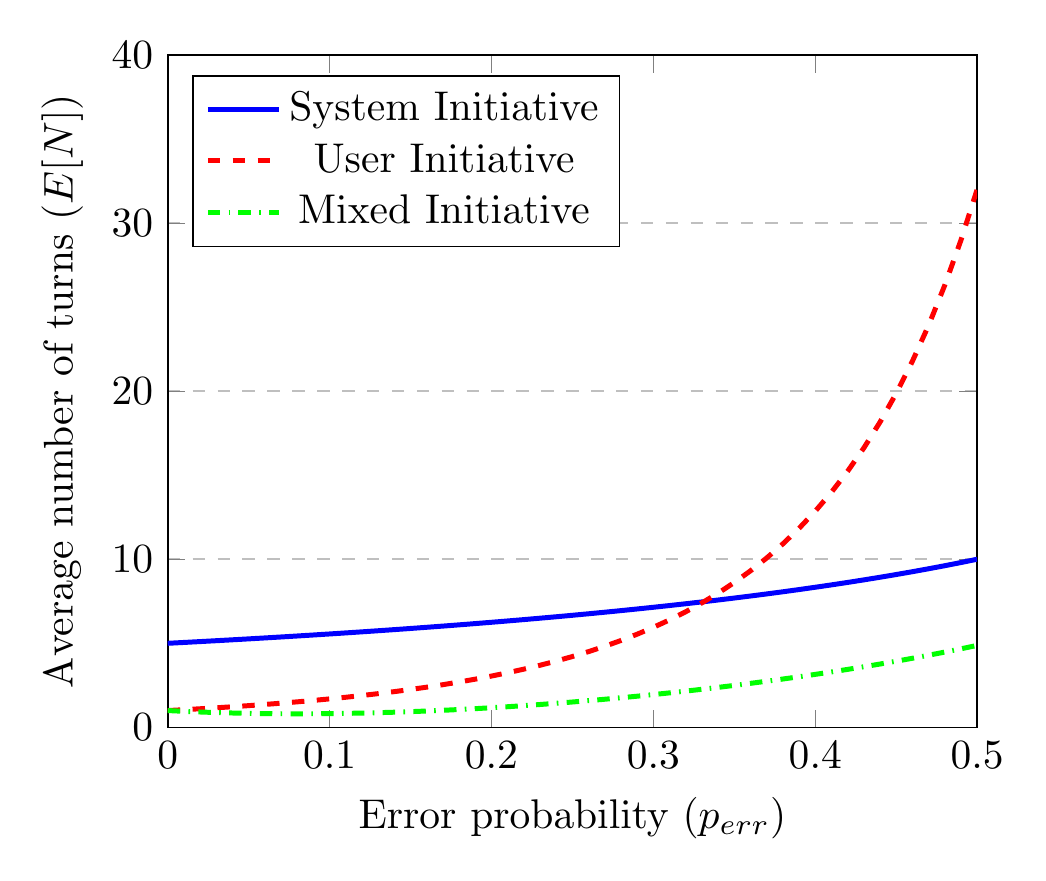
\begin{tikzpicture}[scale=1.5]
				\begin{axis}[
					xlabel={Error probability ($p_{err}$)},
					ylabel={Average number of turns ($\mathbb{E} [N]$)},
					scaled ticks = false,
					tick label style={/pgf/number format/fixed},
					xmin=0, xmax=0.5,
					ymin=0, ymax=40,
					xtick={0,0.1,0.2,0.3,0.4,0.5},
					ytick={0,10,20,30,40},
                                        legend pos=north west,
					ymajorgrids=true,
					grid style=dashed,
          %colorbrewer cycle list=Set2,
				]
				
				\addplot[color=blue,
					solid,
					very thick,
					error bars/.cd,
					y dir=both,
					y explicit,
					]
					coordinates {
					(0,5)
(0.01,5.05050505050505)
(0.02,5.10204081632653)
(0.03,5.15463917525773)
(0.04,5.20833333333333)
(0.05,5.26315789473684)
(0.06,5.31914893617021)
(0.07,5.37634408602151)
(0.08,5.43478260869565)
(0.09,5.49450549450549)
(0.1,5.55555555555556)
(0.11,5.61797752808989)
(0.12,5.68181818181818)
(0.13,5.74712643678161)
(0.14,5.81395348837209)
(0.15,5.88235294117647)
(0.16,5.95238095238095)
(0.17,6.02409638554217)
(0.18,6.09756097560976)
(0.19,6.17283950617284)
(0.2,6.25)
(0.21,6.32911392405063)
(0.22,6.41025641025641)
(0.23,6.49350649350649)
(0.24,6.57894736842105)
(0.25,6.66666666666667)
(0.26,6.75675675675676)
(0.27,6.84931506849315)
(0.28,6.94444444444444)
(0.29,7.04225352112676)
(0.3,7.14285714285714)
(0.31,7.2463768115942)
(0.32,7.35294117647059)
(0.33,7.46268656716418)
(0.34,7.57575757575758)
(0.35,7.69230769230769)
(0.36,7.8125)
(0.37,7.93650793650794)
(0.38,8.06451612903226)
(0.39,8.19672131147541)
(0.4,8.33333333333334)
(0.41,8.47457627118644)
(0.42,8.62068965517242)
(0.43,8.77192982456141)
(0.44,8.92857142857143)
(0.45,9.09090909090909)
(0.46,9.25925925925926)
(0.47,9.43396226415095)
(0.48,9.61538461538462)
(0.49,9.80392156862746)
(0.5,10)
					};
                    
                    \addplot[color=red,
					dashed,
					very thick,
					error bars/.cd,
					y dir=both,
					y explicit,
					]
					coordinates {
					(0,1)
(0.01,1.05153571281335)
(0.02,1.10629161707545)
(0.03,1.16450492244656)
(0.04,1.22643302006977)
(0.05,1.29235543489982)
(0.06,1.36257599015443)
(0.07,1.43742520951759)
(0.08,1.5172629861398)
(0.09,1.60248155139468)
(0.1,1.69350878084303)
(0.11,1.79081188001872)
(0.12,1.89490149859361)
(0.13,2.00633632832981)
(0.14,2.12572824813878)
(0.15,2.25374808871598)
(0.16,2.3911320998183)
(0.17,2.5386892155507)
(0.18,2.69730922732397)
(0.19,2.86797199079244)
(0.2,3.0517578125)
(0.21,3.24985918465773)
(0.22,3.46359406305176)
(0.23,3.69442091425689)
(0.24,3.94395579498235)
(0.25,4.21399176954733)
(0.26,4.50652102244468)
(0.27,4.82376008323414)
(0.28,5.16817865247506)
(0.29,5.542532602331)
(0.3,5.94990182661986)
(0.31,6.39373373583192)
(0.32,6.87789333714593)
(0.33,7.406721012855)
(0.34,7.98509931917638)
(0.35,8.61853037897295)
(0.36,9.31322574615479)
(0.37,10.0762109885347)
(0.38,10.9154476847742)
(0.39,11.8399760787018)
(0.4,12.8600823045268)
(0.41,13.9874949193747)
(0.42,15.2356164932545)
(0.43,16.6197972595141)
(0.44,18.1576593829952)
(0.45,19.869482337893)
(0.46,21.7786623050801)
(0.47,23.9122615317139)
(0.48,26.3016674162993)
(0.49,28.9833859145574)
(0.5,32)


					};
					
											\addplot[color=green,
					dashdotted,
					very thick,
					error bars/.cd,
					y dir=both,
					y explicit,
					]
					coordinates {
					(0,1)
(0.01,0.95346529990505)
(0.02,0.91372479712653)
(0.03,0.880579279457732)
(0.04,0.853836718933333)
(0.05,0.833312269736842)
(0.06,0.818828270570213)
(0.07,0.810214251821505)
(0.08,0.807306947895652)
(0.09,0.809950315105495)
(0.1,0.817995555555556)
(0.11,0.831301147489888)
(0.12,0.849732882618182)
(0.13,0.873163910981609)
(0.14,0.901474793972093)
(0.15,0.934553566176471)
(0.16,0.972295806780952)
(0.17,1.01460472134217)
(0.18,1.06139123480976)
(0.19,1.11257409677284)
(0.2,1.16808)
(0.21,1.22784371345063)
(0.22,1.29180823105641)
(0.23,1.35992493770649)
(0.24,1.43215379402105)
(0.25,1.50846354166667)
(0.26,1.58883193115676)
(0.27,1.67324597429315)
(0.28,1.76170222364445)
(0.29,1.85420708172676)
(0.3,1.95077714285714)
(0.31,2.0514395709942)
(0.32,2.15623251727059)
(0.33,2.26520558136418)
(0.34,2.37842032135758)
(0.35,2.49595081730769)
(0.36,2.6178842944)
(0.37,2.74432181230794)
(0.38,2.87537902823226)
(0.39,3.01118704207541)
(0.4,3.15189333333334)
(0.41,3.29766280058644)
(0.42,3.44867891597242)
(0.43,3.60514500876141)
(0.44,3.76728569417143)
(0.45,3.93534846590909)
(0.46,4.10960547365926)
(0.47,4.29035550995095)
(0.48,4.47792623458462)
(0.49,4.67267666922746)
(0.5,4.875)


					};
                    

				\legend{System Initiative,User Initiative,Mixed Initiative}

				\end{axis}
				\end{tikzpicture}
				\caption{Slot-filling strategies efficiency comparison}
				\label{fig:effcompare}
		\end{figure}

\section{Incremental strategies}
\label{sec:incrstrat}

     Incremental dialogue processing brings a new dimension (a new decision degree of freedom) that can be exploited in order improve the dialogue efficiency. In Chapter \ref{ch:taxonomy}, the following TTP have been selected for implementation: FAIL\_RAW, INCOHERENCE\_INTERP, FEEDBACK\_RAW and BARGE\_IN\_RESP from the user's and the system's perspective. In the following, the ways they can be implemented are discussed.

     The concept of elementary has been proven to be useful for slot-filling strategies analysis. As far as incremental strategies are concerned, analysis is made at a more atomic level since only one dialogue turn is considered. In the following, the user is supposed to have the floor and the system is waiting for her to provide $n_s$ slot values in the same utterance.

     The reader should keep in mind that the architecture used here is the one introduced in Chapter \ref{ch:architecture}, therefore, the Scheduler module is in charge of making turn-taking decisions. It can perform three kinds of actions:

     \begin{itemize}
       \item \textbf{WAIT:} Performed most of the time, it is chosen when the Scheduler decides not to retrieve the service's response at a certain micro-turn, hence waiting for the user to provide more information during the following micro-turns.
       \item \textbf{SPEAK:} The Scheduler decides to commit to the current user's utterance and to provide the corresponding service's response right away. This either translates into a barge-in or an accurate end point detection.
       \item \textbf{REPEAT:} The Scheduler does not retrieve the last service's utterance but the last word of the last user's utterance\footnote{This is a simple way of simulating feedback. In reality, any part of the last partial utterance could be repeated.}. The objective is not to barge-in but perform a feedback that might trigger a reaction from the user or not.
     \end{itemize}

     \paragraph{FAIL\_RAW:} If the user has been holding the floor for too long without providing a single slot value, it might be interesting for the system to interrupt her asking for a reformulation or a repeat. This situation can happen for two main reasons: the user uses off-domain words or expressions (mainly because she is not familiar with the system) or her utterance has been altered because of noise and ASR imperfections. The system can use several criteria in order to decide whether to interrupt the user or not. For example, it can rely on a time threshold: if the user speaks for a period that is larger than that threshold without providing any slot value, then it performs a SPEAK. This duration can be replaced by a number of words or phonemes for example. Consider the following dialogue where the user tries to check his bank account in a noisy environment:

          \begin{dialogue}
            \speak{USER} <noise> like to <noise> number 58 45...
            \speak{SYSTEM} ...Sorry, I don't understand. What can I do for you?
            \speak{USER} Check account number <noise> I repeat, check account 58 45 18 A.
            \speak{SYSTEM} All right, you want to check the account number 58 45 18 A right?
            \speak{USER} Yes.
          \end{dialogue}

          The user is interrupted by the system at the first dialogue turn. If the latter didn't make such a decision, its response would have been the same (\textit{Sorry, I don't understand. What can I do for you?}) as an important part of the request was lost. Therefore, the system barge-in spared the user some time and energy. In this example, the second time the user tries to formulate his request, he does it in a more concise way and repeats it as an effort to make himself clearer. This kind of behaviour have been noticed as a result of a corpus study made in \cite{Ghigi2014}.

     \paragraph{INCOHERENCE\_INTERP:} 
